\documentclass[10pt, a4paper]{article}
\usepackage[paper=a4paper, left=1.5cm, right=1.5cm, bottom=1.5cm, top=3.5cm]{geometry}
\usepackage[utf8]{inputenc}
\usepackage[T1]{fontenc}
\usepackage[spanish]{babel}
\usepackage{indentfirst}
\usepackage{fancyhdr}
\usepackage{latexsym}
\usepackage{lastpage}
\usepackage{calc}
\usepackage{caratula}
\usepackage{fancyhdr}
\usepackage[pdftex]{graphicx}
\usepackage{color}
\usepackage{dsfont}
\usepackage{xspace}
\usepackage{xargs}
\usepackage{listings} 	
\usepackage{algpseudocode}
\usepackage{graphicx}
\usepackage{amsmath}
\usepackage{caption}
\usepackage{amssymb}
\usepackage{float}
\usepackage{sidecap}
\usepackage{textcomp}
\usepackage{wrapfig}
\usepackage{blkarray}
\def\Big#1{\makebox(0,0){\huge#1}}

\titulo{Trabajo Práctico 1: CQTDAH}
\fecha{10 / 4 / 2014}
\materia{Métodos Numéricos}
\grupo{Grupo: Nombre Pendiente}
\integrante{Rama, Roberto}{490/11}{bertoski@gmail.com}
\integrante{Vanotti, Marco}{229/10}{mvanotti@dc.uba.ar}
\integrante{Ventura, Alejandro}{249/11}{vn2.amv@gmail.com}

\def\contentsname{Índice}

\begin{document}

\maketitle

\tableofcontents

\pagestyle{fancy}
\lhead{Rama, Vanotti, Ventura}
\rhead{Métodos Numéricos - TP1}

\clearpage
\section{Introducción}
  \subsection{Objetivos}
El objetivo principal del presente trabajo es la estimaci\'on de las temperaturas internas a la pared de un alto horno (horno de fundición de metales), para poder así determinar la posición aproximada de la isoterma de temperatura 'iso', y poder estudiar el estado y fiabilidad del horno. 
Se busca adem\'as comparar la eficiencia de distintos m\'etodos computacionales para la obtención de dicha isoterma, para el caso en que hay que realizar una medición \'unica de la temperatura del horno, o varias.

\subsection{Introducción}
El fen\'omeno físico de transmisión del calor es descripto detalladamente en la conocida ecuación del calor, para el caso en el que solo se desea conocer el equilibrio final de temperaturas de un sistema, se puede disponer de ecuaciones mas sencillas, estas ecuaciones de estado dependen de las caracter\'isticas del sistema, y del tipo de coordenadas usadas. Nuestro caso consiste de un sistema físico en forma de 'disco', medido en coordenadas polares, esto es, con las variables r y $\theta$. La ecuación que describe la temperatura para cada par $(r, \theta)$ en este sistema es una ecuación de segundo orden, en derivadas parciales:

$$\frac{\delta ^{2} T(r, \theta)}{\delta r^{2}} + \frac{1}{r} \frac{\delta T (r,\theta)}{\delta r} + \frac{1}{r^{2}} \frac{\delta^{2} T(r,\theta)}{\delta \theta ^{2}} = 0$$

~

~

Como los fen\'omenos y modelos físicos tienen una naturaleza continua mientras que los modelos computacionales tienen una naturaleza discreta, los mismos crean la necesidad de realizar un proceso de discretizaci\'on sobre el modelo físico inicial y una interpolación para refinar la solución encontrada.
\\
Para la discretización de la ecuación se utilizan formulas de diferencias finitas, que son versiones discretas de la definición continua de derivada. Se hacen aproximaciones discretas a la variable radio. Así se puede transformar una ecuación diferencial de estas caracter\'isticas en un sistema de ecuaciones lineales.
\\
Como m\'etodo de interpolación, se puede utilizar una función lineal que una los puntos $(r_{i}, t_{i})$ y $(r_{i+1}, t_{i+1})$ del dominio. A esta función luego se le calcula la inversa, con lo cual para cada temperatura (fijado el \'angulo), devuelve un valor que representa al radio (entre $r_{i}$ y $r_{i+1}$)  correspondido con esa temperatura.

~

Luego usaremos la discretizaci\'on antes descripta para obtener un sistema de ecuaciones lineales que resolveremos mediante eliminaci\'on Gaussiana y factorizaci\'on LU. La eliminación Gaussiana es un algoritmo para la resolución de sistemas de ecuaciones lineales de la forma $Ax=b$, donde A es una matriz que representa los coeficientes de las variables del sistema, x es el vector inc\'ognita, y b el vector termino independiente. El m\'etodo consiste en la obtenci\'on de una matriz triangular mediante la realización de operaciones elementales en una matriz que representa el sistema de ecuaciones. Una vez triangulada la matriz se procede a hacer la substitución hacia atr\'as (backward substitution).
La complejidad del algoritmo es de $\mathcal{O}(n^{3})$ sobre el tamaño de la matriz, si bien las operaciones de la substitución pueden realizarse solo en $\mathcal{O}(n^{2})$.
\\
\\
Un m\'etodo para optimizar el procedimiento cuando tenemos varias instancias (distintas mediciónes y por lo tanto distinto vector termino independiente) a resolver relacionadas por el mismo modelo físico (sin alterar la matriz caracter\'istica) es la factorización LU (Lower, Upper) de la matriz. La misma consiste en escribir a la matriz inicial como el producto de una matriz triangular inferior y otra triangular superior, llamadas L y U respectivamente. 
\\
Con esto la ecuación vectorial del sistema inicial es equivalente a $LUx=b$, pudiendo escribirse como dos ecuaciónes distintas, llamando '$y$' a '$Ux$', como $Ly=b$ y $Ux = b$. Al ser las matrices de estas ecuaciónes, triangulares no hace falta la utilización de la eliminación Gaussiana, solamente la substitución hacia atr\'as. Con este m\'etodo se espera conseguir una complejidad de $\mathcal{O}(n^{2})$ una vez realizada la factorización, lo que podría mejorar el rendimiento, a la hora de realizar varias mediciones con un mismo modelo físico.




\clearpage
\section{Desarrollo}
  \subsection{Construcci\'on del modelo}

Sean $r_e, r_i \in \mathcal{R}$ el radio exterior de la pared del horno y el radio interno respectivamente. Llamaremos $T(r,\theta)$ a la temperatura en el punto dado por las coordenadas polares $(r,\theta)$, siendo $r$ el radio y $\theta$ el \'angulo polar de dicho punto. En estado estacionario, esta temperatura satisface la ecuaci\'on de calor:

~

\begin{equation}
 \frac{\partial T(r,\theta)}{\partial r^2} + \frac{1}{r} \frac{\partial T(r,\theta)}{\partial r} + \frac{1}{r^2} \frac{\partial^2T(r,\theta)}{\partial\theta^2} = 0
\end{equation}

~

Si llamamos $T_i \in \mathcal{R}$ a la temperatura en el interior del horno y $T_e:[0,2\pi] \rightarrow \mathcal{R}$ a la funci\'on de temperatura en el borde exterior del horno (correspondiente a los sensores) tendremos que $T(r,\theta) = T_i$ para todo punto $(r,\theta)$ con $r \leq r_i$ y que $T(r_e, \theta) = T_e(\theta)$ para todo punto $(r_e, \theta)$.

~

Para construir nuestro modelo y lograr una resoluci\'on computacional comenzaremos con una discretizaci\'on del dominio del problema a resolver, ya que el mismo en la vida real tiene infinitos radios y \'angulos. Consideraremos las siguientes particiones:

\begin{itemize}
 \item $0 = \theta_0 < \theta_1 < ... < \theta_n = 2 \pi$ en $n$ \textbf{\'angulos} discretos con $\theta_k - \theta_{k-1} = 2\pi/n = \Delta\theta$ para $k = 1,...,n$.
 \item $r_i = r_0 < r_1 < ... < r_m = r_e$ en $m$ \textbf{radios} discretos con $r_j - r_{j-1} = (r_i - r_e)/(m-1) = \Delta r$ para $j=1,...,m$.
\end{itemize}

Es importante remarcar que la discretizaci\'on de los \'angulos esta en limitada por la cantidad de sensores que tendremos en el horno real, no pudiendo superar a la cantidad de los mismos ya que ser\'an nuestros datos de entrada.

Una vez discretizados los valores de las coordenadas polares el problema ahora consiste en determinar el valor de la funci\'on $T$ en los puntos $(r_j, \theta_k)$. Llamemos $t_{jk} = T(r_j, \theta_k)$ al valor de la funci\'on $T$ en el punto $(r_j, \theta_k)$, cuyos valores son desconocidos. Aproximaremos las derivadas de la ecuaci\'on (1) de la siguiente manera:

~

\begin{equation}
 \frac{\partial T(r,\theta)}{\partial r^2}(r_j,\theta_k) \cong 
 \frac{t_{j-1,k}-2t_{j,k}+t_{j+1,k}}{(\Delta r)^2}
\end{equation}

\begin{equation}
 \frac{\partial T(r,\theta)}{\partial r}(r_j,\theta_k) \cong
 \frac{t_{j,k}-t_{j-1,k}}{\Delta r} 
\end{equation}

\begin{equation}
 \frac{\partial^2T(r,\theta)}{\partial\theta^2}(r_j,\theta_k) \cong
 \frac{t_{j,k-1}-2t_{j,k}+t_{j,k+1}}{(\Delta \theta)^2}
\end{equation}

~

~

Si reemplazamos las aproximaciones (2), (3) y (4) en (1) obtendremos:

~

\begin{equation}
 \frac{t_{j-1,k}-2t_{j,k}+t_{j+1,k}}{(\Delta r)^2} 
 + \frac{t_{j,k}-t_{j-1,k}}{r(\Delta r)} 
 + \frac{t_{j,k-1}-2t_{j,k}+t_{j,k+1}}{r^2(\Delta \theta)^2}
 = 0
\end{equation}

~

~

Para cada punto $(r_j,\theta_k)$, lo que nos deja con un sistema de ecuaciones lineales que modela el problema discretizado.

\newpage
\subsection{Idea de resoluci\'on}

La idea es resolver el sistema de ecuaciones en un primer lugar represent\'andolo en matrices y luego utilizando eliminaci\'on Gaussiana y factorizaci\'on LU para resolver el mismo. El sistema quedar\'a de la forma $At = b$ siendo $t$ y $b$ vectores columna  en donde $A$ contendr\'a a los coeficientes de la ecuaci\'on de calor (5), $b$ contendr\'a los datos para resolver el sistema y $t$ contendr\'a cada punto interno del horno correspondiente con la discretizaci\'on.

~

Los vectores columna $t$ y $b$ tendr\'an ambos dimensi\'on $nm$. La estructura de $t$ estar\'a conformada por los valores $t_{1,1}, t_{1,2}, ..., t_{1,n}, t_{2,1} ..., t_{m,n}$ dispuestos en forma de columna. Por otro lado, el vector $b$ tendr\'a el valor $1500$ en las primeras $n$ posiciones (correspondientes al radio interno del horno), ceros en las siguientes $m(n-2)$ posiciones y los valores correspondientes a $T_e(\theta_1), T_e(\theta_2), ..., T_e(\theta_n)$ en las \'ultimas $n$ posiciones (correspondientes a los valores de los sensores).

~


 \begin{equation*}
\left( \begin{array}{ccccccc}
1 & 0 & 0 & 0 & 0 & \dots & 0\\
0 & 1 & 0 & 0 & 0 & \dots & 0\\
\vdots & & \ddots & & & & \vdots\\
0  & \dots & 0 & 1 & 0 & \dots  & 0\\

  & \dots &  & t_{i,j-1} & t_{i,j} & \dots &\\

\vdots & & & \vdots & & & \vdots\\
0  & \dots & & 0 & & \dots  & 1\\
\end{array} \right)
\left( \begin{array}{c}
t_{1,1} \\
t_{1,2} \\
\vdots \\
t_{1,n} \\
t_{2,1} \\
\vdots \\
t_{m,n} \\ \end{array} \right)
= \left( \begin{array}{c}
1500 \\
1500 \\
\vdots \\
1500\\
0\\
\vdots\\
T_e(\theta_n)\end{array} \right)
\end{equation*}

~

~

La matriz $A$ por otro lado ser\'a cuadrada de tama\~no $nm$ en cada dimensi\'on. Las primeras $n$ filas ser\'an una identidad que se corresponder\'a con las temperaturas en el radio interno, que como son dato las conocemos. Las siguientes $m(n-2)$ filas corresponder\'an a las ecuaciones de calor por cada punto interno de la discretizaci\'on. Cada ecuaci\'on tendr\'a $nm$ t\'erminos (aunque la mayor\'ia de ellos acompa\~nados por un coeficiente nulo) por lo que la matriz tendr\'a $nm$ columnas. Finalmente en las ultimas $n$ filas de la matriz se encontrar\'a la identidad que se corresponder\'a con las temperaturas externas, es decir aquellas registradas por los sensores.

~

Ahora solamente nos falta saber como llenar $A$. Si hacemos un manejo algebraico sobre la ecuaci\'on (5) juntando los elementos iguales nos queda que:

\begin{equation*} \implies
 \frac{t_{j-1,k}}{(\Delta r)^2}
 -\frac{2t_{j,k}}{(\Delta r)^2}
 +\frac{t_{j+1,k}}{(\Delta r)^2}
 +\frac{t_{j,k}}{r(\Delta r)}
 -\frac{t_{j-1,k}}{r(\Delta r)}
 +\frac{t_{j,k-1}}{r^2(\Delta \theta)^2}
 -\frac{2t_{j,k}}{r^2(\Delta \theta)^2}
 +\frac{t_{j,k+1}}{r^2(\Delta \theta)^2} = 0
\end{equation*}

\begin{equation*} \implies
 \frac{t_{j,k}}{r(\Delta r)}
 -\frac{2t_{j,k}}{(\Delta r)^2}
 -\frac{2t_{j,k}}{r^2(\Delta \theta)^2}
 +\frac{t_{j-1,k}}{(\Delta r)^2}
 -\frac{t_{j-1,k}}{r(\Delta r)}
 +\frac{t_{j+1,k}}{(\Delta r)^2}
 +\frac{t_{j,k-1}}{r^2(\Delta \theta)^2}
 +\frac{t_{j,k+1}}{r^2(\Delta \theta)^2} = 0
\end{equation*}

~

~

Es decir que me queda para la ecuaci\'on correspondiente a cada $t_{j,k}$:

\begin{figure}[!htb]
\centering
\minipage{0.5\textwidth}
  \begin{equation}
  c_1 = c_{j,k} = \frac{1}{r\Delta r}-\frac{2}{(\Delta r)^2}-\frac{2}{(r\Delta \theta)^2}
  \end{equation}

  \begin{equation}
  c_2 = c_{j-1,k} = \frac{1}{(\Delta r)^2}-\frac{1}{r\Delta r}
  \end{equation}

  \begin{equation}
  c_3 = c_{j+1,k} = \frac{1}{(\Delta r)^2}
  \end{equation}

  \begin{equation}
  c_4 = c_{j,k-1} = c_{j,k+1} = \frac{1}{(r\Delta \theta)^2}
  \end{equation}
\endminipage\hfill
\minipage{0.5\textwidth}
  
  $$r = r_i + (j-1)(\Delta r)$$
  
  $$\Delta \theta = 2\pi/n$$
  
  $$\Delta r = (r_i-r_e)/(m-1)$$
  
\endminipage\hfill
\end{figure}

Finalmente para llenar $A$ la inicializaremos en cero y luego nos moveremos por la diagonal. Si estamos en alguna de las dos \'areas de identidad, es decir las primeras o \'ultimas $n$ filas, pondremos un $1$. De lo contrario asignaremos el valor correspondiente a $c_{j,k}$ para el $j$ y $k$ apropiados y los otros $4$ valores en las posiciones correspondientes. En los casos en modificamos $j$ nos moveremos $n$ columnas hacia la izquierda si restamos y hacia la derecha si sumamos. En los casos en los que $k+1$ o $k-1$ se salgan fuera del rango $[1,n]$ le aplicaremos m\'odulo $n$, moviendonos as\'i $n-1$ columnas hacia la izquierda o derecha respectivamente.

%TODO: Imagen explicativa de esto ^^^

\newpage
\subsection{Algoritmos}

\begin{figure}[!htb]
\centering
\minipage{0.5\textwidth}
  \begin{algorithmic}[1]
  \Function{WithFifteenThetas}{$r_i$, $r_e$, $n$, $m$, $T_i$, $T_e$}
    \State $dr \leftarrow (r_e - r_i) / (m - 1)$
    \State $dt \leftarrow 2\pi/n$
    \State \textbf{Matrix} $b \in \mathcal{R}^{nm\times 1}, A\in \mathcal{R}^{nm\times nm}$
    \For{$i \in [1,nm]$}
      \State $b[i][1] \leftarrow T_i[i]$
      \State $b[nm-i][1] \leftarrow T_e[i]$
    \EndFor
    \State $j \leftarrow 1, k \leftarrow 1$
    \For{$i \in [1,nm]$}
      \If{$i \in [1,n] \vee i \in [(n-1)m,nm]$}
	\State $A[i][i] \leftarrow 1$
      \Else
	
	\State $A[i][i] \leftarrow c_1(j, r_i, dr, dt)$
	\State $A[i][i-n] \leftarrow c_2(j, r_i, dr, dt)$
	\State $A[i][i+n] \leftarrow c_3(j, r_i, dr, dt)$
	
	\If{$k=n$}
	  \State $A[i][i-n+1] \leftarrow c_4(j, r_i, dr, dt)$
	\Else
	  \State $A[i][i+1] \leftarrow c_4(j, r_i, dr, dt)$
	\EndIf
	
	\If{$k=1$}
	  \State $A[i][i+n-1] \leftarrow c_4(j, r_i, dr, dt)$
	\Else
	  \State $A[i][i-1] \leftarrow c_4(j, r_i, dr, dt)$
	\EndIf

	\State $k \leftarrow k+1$      
	\If{$k>n$}
	  \State $j \leftarrow j+1, k \leftarrow 1$
	\EndIf
	
      \EndIf
    \EndFor
    \State \Return $solve(A,b)$
  \EndFunction
  \end{algorithmic} 
  
  ~
  
  \begin{algorithmic}[1]
    \Function{BackSub}{\textbf{Matrix} $A$, \textbf{Matrix} $b$}
      \State \textbf{Matrix} $R \in \mathcal{R}^{cols(A)\times 1}$
      
      \For{$i \in [A.n, 1]$}
	 \If{$a_{i,i} \not= 0$}
	    \State $r_{i,1} \leftarrow (b_{i,1} - A[i] \times R) / a_{i,i}$
	 \EndIf
      \EndFor
      
      \State \Return $R$
    \EndFunction
  \end{algorithmic}   
  
  ~
  
  \begin{algorithmic}[1]
    \Function{ForwSub}{\textbf{Matrix} $A$, \textbf{Matrix} $b$}
      \State \textbf{Matrix} $R \in \mathcal{R}^{cols(A)\times 1}$
      
      \For{$i \in [1, A.n]$}
	 \If{$a_{i,i} \not= 0$}
	    \State $r_{i,1} \leftarrow (b_{i,1} - A[i] \times R) / a_{i,i}$
	 \EndIf
      \EndFor
      
      \State \Return $R$
    \EndFunction
  \end{algorithmic} 
  
\endminipage\hfill
\minipage{0.01\textwidth}
\endminipage\hfill
\minipage{0.49\textwidth}

\textbf{WithFifteenThetas} es la funci\'on principal encargada de la resoluci\'on de una instancia del problema. Consideramos con fines pr\'acticos que ya recibe los datos procesados del input por los par\'ametros de radio interno ($r_i$), radio externo ($r_e$), cantidad de \'angulos ($n$), cantidad de radios ($m$), un vector de temperaturas internas ($T_i$) y un vector de temperaturas externas ($T_e$).  

~

Entre las lineas 2 a 9 se inicializan los valores de $\Delta r$ ($dr$) y $\Delta \theta$ ($dt$) y se carga el vector columna $b$ con los valores provenientes de $T_i$ y $T_e$, quedando en los $n$ primeros lugares los valores de $T_i$ y en los $n$ \'ultimos los valores de $T_e$. En la linea 9 se puede observar la inicializaci\'on de los contadores $j$ y $k$. Entre las lineas 10 a 32 tenemos el bucle responsable de llenar la matriz $A$. Como explicamos en la secci\'on anterior, la idea es moverse por la diagonal y si se encuentra en un \'area identidad asignar un $1$ (lineas 11 y 12). De lo contrario, asignaremos el coeficiente $c_1$ a la posici\'on de la diagonal y $c_2$, $c_3$ y $c_4$ a las columnas correspondientes de esa misma fila. Los coeficientes son calculados como se los muestra en las formulas (6), (7), (8) y (9). 

Finalmente en la linea 33 se llama a la funci\'on solve que resuelve el sistema lineal. En nuestra implementaci\'on en ese momento se llama a solveGE (resoluci\'on por eliminaci\'on Gaussiana) o solveLU (resoluci\'on por factorizaci\'on LU) dependiendo del modo en el que se este usando el programa. Para simplicidad del pseudoc\'odigo decidimos dejar fuera dicho detalle ya que pertenece mas a la implementaci\'on. El llenado de la matriz $A$ tiene una complejidad de $\mathcal{O}(nm)$.

~

\textbf{BackSub} (backSubstitution) y \textbf{ForwSub} (forwardSubstitution) realizan la resoluci\'on de un sistema con una matriz $A$ diagonal superior y diagonal inferior respectivamente. En \textbf{BackSub} en la linea 2 se inicializa con ceros el vector columna en donde se devolver\'a el resultado. Luego entre las lineas 3 a 7, se procede a iterar movi\'endose por la diagonal. Si se encuentra un cero se saltea esa fila (linea 4), ya que de haberse encontrado toda la fila es cero. De lo contrario en la linea 5 se multiplica la fila $i$ de $A$ ($A[i]$) por el vector resultado ($R$), se lo resta a el dato correspondiente a esa ecuaci\'on y se lo divide por el coeficiente de la inc\'ognita que se quiere despejar. 

Si nos detenemos a observar esta \'ultima operaci\'on, podremos ver que lo que se esta haciendo es encontrar el valor de $x_i$ despejando la ecuaci\'on $a_{i,i}x_i + A[i] \times R = b_{i,1}$ en donde $A[i] \times R$ es la suma de los $x_i$ conocidos por sus constantes. En la linea 8 el algoritmo devuelve el resultado, que una vez terminadas las iteraciones contendr\'a los valores que resuelven el sistema ordenados de forma $x_1, x_2, ..., x_{cols(A)}$. \textbf{BackSub} tiene una complejidad de $\mathcal{O}(n^2)$.

~

\textbf{ForwSub} tiene un comportamiento isomorfo a \textbf{BackSub}, la \'unica diferencia es que comienza despejando la primera ecuaci\'on en lugar de la \'ultima y sigue desde all\'i hasta la \'ultima. 


\endminipage\hfill
\end{figure}

\newpage
\begin{figure}[!htb]
\centering
\minipage{0.5\textwidth}
  
  \begin{algorithmic}[1]
    \Function{SolveGE}{\textbf{Matrix} $A$, \textbf{Matrix} $b$}    
      \For{$i \in [1, A.m)$}
	\For{$z \in [i+1, A.m]$}
	   \State $A[z] \leftarrow A[z] - (a_{z,i}/a_{i,i})\cdot A[i]$
	   \State $b[z] \leftarrow (-a_{z,i}/a_{i,i})\cdot b[i]$
	\EndFor
      \EndFor
      \State \Return $backSub(A,b)$
    \EndFunction
  \end{algorithmic} 
  
  ~
  
  ~
  
  \begin{algorithmic}[1] 
    \Function{SolveLU}{\textbf{Matrix} $A$, \textbf{Matrix} $b$}
      \State \textbf{Matrix} $LU \leftarrow decompLU(A)$
      \State \textbf{Matrix} $y \leftarrow forwSub(LU.first,b)$
      \State \Return $backSub(LU.second,y)$
    \EndFunction
  \end{algorithmic}
  
  ~
  
  ~
  
  \begin{algorithmic}[1]
    \Function{DecompLU}{\textbf{Matrix} $A$}
      \State \textbf{Matrix} $L \in \mathcal{R}^{nm\times nm}$
      \State \textbf{Matrix} $U \in \mathcal{R}^{nm\times nm}$
      
      \For{$i \in [1, A.m)$}
	\For{$z \in [i+1, A.m]$}
	    \State $l_{z,i} \leftarrow a_{z,i}/a_{i,i}$
	    \State $U[z] \leftarrow A[z] - (a_{z,i}/a_{i,i})\cdot A[i]$
	\EndFor
	\State $l_{i,i} \leftarrow 1$
      \EndFor
      \State $L[A.m][A.m] \leftarrow 1$
      
      \State \Return <$L,U$>
    \EndFunction
  \end{algorithmic} 
  
\endminipage\hfill
\minipage{0.01\textwidth}
\endminipage\hfill
\minipage{0.49\textwidth}

\textbf{SolveGe} (solverGaussianElimination) utiliza la eliminaci\'on Gausseana para diagonalizar superiormente el sistema y luego lo resuelve utilizando backSubstitution. En nuestro algoritmo, en las lineas 2 y 3 a 6 y 7 se pueden observar los for principales del mismo. El primer for, cuyo contador es $i$, se encarga de apuntar a la fila que se esta usando para conseguir ceros en las dem\'as. El segundo for, a quien el contador $j$ le pertenece, se encarga de iterar por las filas inferiores a la fila $i$. 

En cada iteraci\'on se le resta a la fila $z$ un m\'ultiplo de la fila $i$, de forma tal que se origine un cero en la posici\'on $(z,i)$ (linea 4). En la linea 5 se repite dicha operaci\'on con el vector columna $b$, de forma tal de conservar la concordancia con el sistema original. Una vez terminada la iteraci\'on completa del segundo for, los \'unicos lugares en donde habr\'an valores distintos de cero en la columna $i$, ser\'a en arriba de la diagonal. Finalmente con la matriz diagonalizada superiormente se utiliza el algoritmo de backSub para devolver una resoluci\'on al sistema. La complejidad de la eliminaci\'on Gausseana es de $\mathcal{O}(n^3 + n^2) \subseteq \mathcal{O}(n^3)$.

~

\textbf{SolveLU} utiliza la factorizaci\'on LU para separar el sistema original en dos sistemas que juntos son equivalentes al original. Al separarlos, una de de las matrices queda diagonalizada de forma inferior (L) y la otra de forma superior (U). Luego se puede resolver el sistema utilizando forwardSubstitution para el sistema inferior y backSubstitution para el sistema superior. La ventaja de este m\'etodo es que el vector columna $b$ no es modificado en la diagonalizaci\'on y por lo tanto podremos guardarnos las matrices $L$ y $U$ para resolver sistemas con un $b$ distinto ahorr\'andonos el costo de la diagonalizaci\'on.

\endminipage\hfill
\end{figure}

La funci\'on \textbf{DecompLU} sirve para descomponer una matriz $A$ en dos matrices $L$ y $U$ de forma tal que se cumpla que $L\cdot U = A$. Es b\'asicamente una eliminaci\'on Gausseana que guarda en la matriz $L$ los coeficientes que se van utilizando en cada paso (linea 6), adem\'as de colocarle en la diagonal todos unos (linea 9 y 11). Una vez terminada la diagonalizaci\'on devuelve una tupla con ambas matrices. 


\begin{SCfigure}[1][ht!]
\sidecaptionvpos{figure}{t}
  \caption{ Realizando un spy en Matlab luego de llenar la matriz con el algoritmo propuesto anteriormente pudimos visualizar que su llenado era correcto. En la imagen se pueden observar aproximadamente las primeras 70 filas y columnas de la matriz, en las que se aprecia la identidad en las primeras filas y luego la forma caracter\'istica que deber\'ia tener por las coordenadas polares involucradas y sus saltos de columnas al restarse o sumarse a alguna de ellas.\newline\newline\newline\newline\newline\newline}
  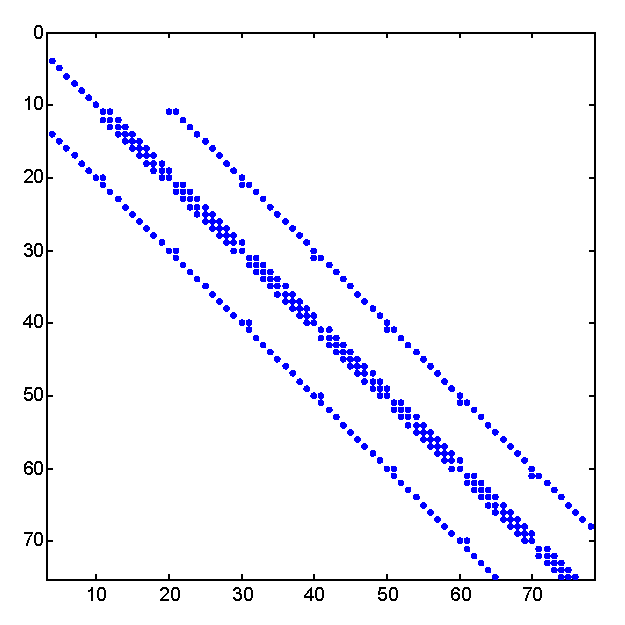
\includegraphics[width=0.4\textwidth]{figures/spy.pdf}
  \label{compbench-glu}
\end{SCfigure}

\newpage

En nuestra implementaci\'on este algoritmo funciona modificando solamente $A$ con el objetivo de ahorrar memoria. Esto se logra eliminando las lineas 11 y 9, haciendo las asignaciones a $A$ en vez de a $L$ y $U$ en las lineas 6 y 7 y devolviendo $A$ en vez de la tupla. Obviamente esta \'ultima modificaci\'on repercute tambi\'en en la funci\'on \textbf{SolveLU}, en la cual hacemos modificaciones en los algoritmos de \textbf{ForwSub} y \textbf{BackSub} para que solamente se muevan por ciertos \'indices de $A$ en cada caso, a forma de calcular correctamente la resoluci\'on de cada sistema sin la necesidad de utilizar dos matrices distintas. El motivo por el cual presentamos esta versi\'on mas b\'asica es porque es mas elegante y f\'acil de entender que su versi\'on optimizada.

~

La complejidad de \textbf{DecompLU} es de $\mathcal{O}(n^3)$, lo que desemboca en una complejidad de $\mathcal{O}(n^3 + 2n^2) \subseteq \mathcal{O}(n^3)$ para \textbf{SolveLU}. Sin embargo, es importante remarcar que si hacemos resoluciones del mismo sistema con la factorizaci\'on LU solamente deberemos resolver los sistemas diagonalizados, por lo que el costo de \textbf{SolveLU} se reduce a $\mathcal{O}(2n^2) \subseteq \mathcal{O}(n^2)$ para las resoluciones sucesivas a la primera. Finalmente podemos ver que \textbf{WithFifteenThetas} tiene una complejidad total de $\mathcal{O}(nm + (nm)^3) \subseteq \mathcal{O}((nm)^3)$ con \textbf{SolveGE} y con la primera resoluci\'on de \textbf{SolveLU}. Sin embargo, las sucesivas resoluciones con \textbf{SolveLU} del mismo sistema tienen una complejidad de $\mathcal{O}((nm)^2)$.

\begin{figure}[!htb]
\centering
\minipage{0.5\textwidth}

\begin{algorithmic}[1]
    \Function{getIsoterm}{\textbf{Vector} $T$, $n$, $m$, $iso$}
      \State \textbf{Vector} $res \in \mathcal{R}^{n}$

      \For{$k \in [0, n)$}
	  \State{\textbf{int} best $\leftarrow$ 0}

	  \For{$j \in [0, m)$}
	      \State {best $\leftarrow$ j}
	      \If{$T[j * n + k][0] < iso$}
		  \State \textbf{break}
	      \EndIf
	  \EndFor

	  \State{\textbf{double} dr $\leftarrow$ $\frac{r_e - r_i}{m - 1}$}

	  \If{best $\geq m $}
	      \State{$res_{k} \leftarrow r_e$}
	      \State{continue}
	  \EndIf

	  \State{$r_2 \leftarrow best$}
	  \State{$r_1 \leftarrow best - 1$}

	  \State{$t_1 = T[r_1 * n + k][0]$}
	  \State{$t_2 = T[r_2 * n + k][0]$}
	  \State{$res_{k} \leftarrow (isovalue - t_1) * \frac{r_2 - r_1}{t_2 - t_1} + r_1$}

	  \State{$res_{k} \leftarrow res_{k} * dr$}
	  \State{$res_{k} \leftarrow res_{k} + r_i$}
    \EndFor
    
    \State \Return $res$
  \EndFunction
\end{algorithmic}   

\endminipage\hfill
\minipage{0.01\textwidth}
\endminipage\hfill
\minipage{0.49\textwidth}

Finalmente, \textbf{getIsoterm} es la función que calcula la curva isoterma. Toma como argumentos la matriz de temperaturas, la cantidad de \'angulos y radios, y el valor de temperatura buscado. Luego devuelve un vector con los radios por los que pasa la curva para cada \'angulo $\theta$.
En la linea 2 se encuentra el ciclo principal, que se encarga de recorrer los \'angulos, para poder calcular el radio por el cual pasa la isoterma  en cada \'angulo por separado.  El ciclo de la linea 5 se encarga de recorrer radialmente en dicho \'angulo hasta que la temperatura sea menor que la isoterma buscada (aquí se asume que avanzando radialmente, las temperaturas solo pueden disminuir), con lo cual el radio buscado esta entre este radio, el j-ésimo y el anterior.  Estos valores luego son guardados en la variable '$r_2$' y '$r_1$', y sus temperaturas en $t_2$ y $t_1$ respectivamente.
Para interpolar se usa la inversa de una recta, que pasa por los puntos ($r_1$, $t_1$) y ($r2$, $t2$). Dicha recta, dentro de su dominio $[r_1,r_2]$, trabajar\'ia como una función interpoladora que devuelve la temperatura, dado un radio. Pero al usar su inversa, sucede que al dar el valor de una temperatura (que en este caso sera siempre el de la isoterma), devuelve el radio del que provino. Este valor es asignado a $res_{k}$ y luego multiplicado por delta r y adicionado a $r_{i}$ para que represente el valor del radio real.
Aquí termina el ciclo principal y se realiza el calculo nuevamente para el siguiente \'angulo, hasta recorrerlos todos. La función retorna el vector de radios de la isoterma por el vector '$res$'.

\endminipage\hfill
\end{figure}




\clearpage
\section{Experimentación}
  \subsection{Instancias propuestas}

En la siguiente sección analizaremos tres instancias distintas del sistema.

Estas consisten en:
\begin{itemize}
    \item{Un horno muy frío (temperatura interior: 1500, temperatura exterior: 30)}
    \item{Un horno muy caliente (temperatura interior: 1500, temperatura exterior: 480)}
    \item{Un horno averiado, que para la mitad superior esté muy caliente y para la mitad inferior muy frío}
\end{itemize}

Para todos los casos, la isoterma buscada es de 500 grados.

La utilidad de estos tres casos es para mostrar que el tiempo de resolución del sistema no depende de los valores del mismo, sino de cómo se discretiza el horno. El tercer caso nos resulta interesante, además, para ver cómo varía la isoterma al tener tan marcada la diferencia de temperatura. 

\subsection{Análisis de isoterma}

En la figura \ref{exp1-hfhc} podemos ver un gráfico de los hornos y su respectiva isoterma. Previamente explicamos cómo se calcula esta isoterma y en los gráficos podemos ver esto reflejado. Para el horno caliente, podemos observar que la isoterma está cerca de las paredes. Esto es porque las paredes externas tienen una temperatura de $480$. Para el horno chico, vemos que la isoterma se encuentra más bien lejos de las paredes externas, pues estas se encuentran frías.  

\begin{figure}[!htb]
    \caption{Izquierda: Horno Caliente, Derecha: Horno Frío}
    \label{exp1-hfhc}
\centering
\minipage{0.5\textwidth}

  \includegraphics[width=1\textwidth]{figures/calor-isoterma-mn19.pdf}

\endminipage\hfill
\minipage{0.5\textwidth}

  \includegraphics[width=1\textwidth]{figures/frio-isoterma-mn19.pdf}

\endminipage\hfill
\end{figure}

\clearpage
\begin{figure}[!htb]
    \caption{Horno con parte inferior caliente y parte superior fría}
    \label{exp1-hfc}
\centering
  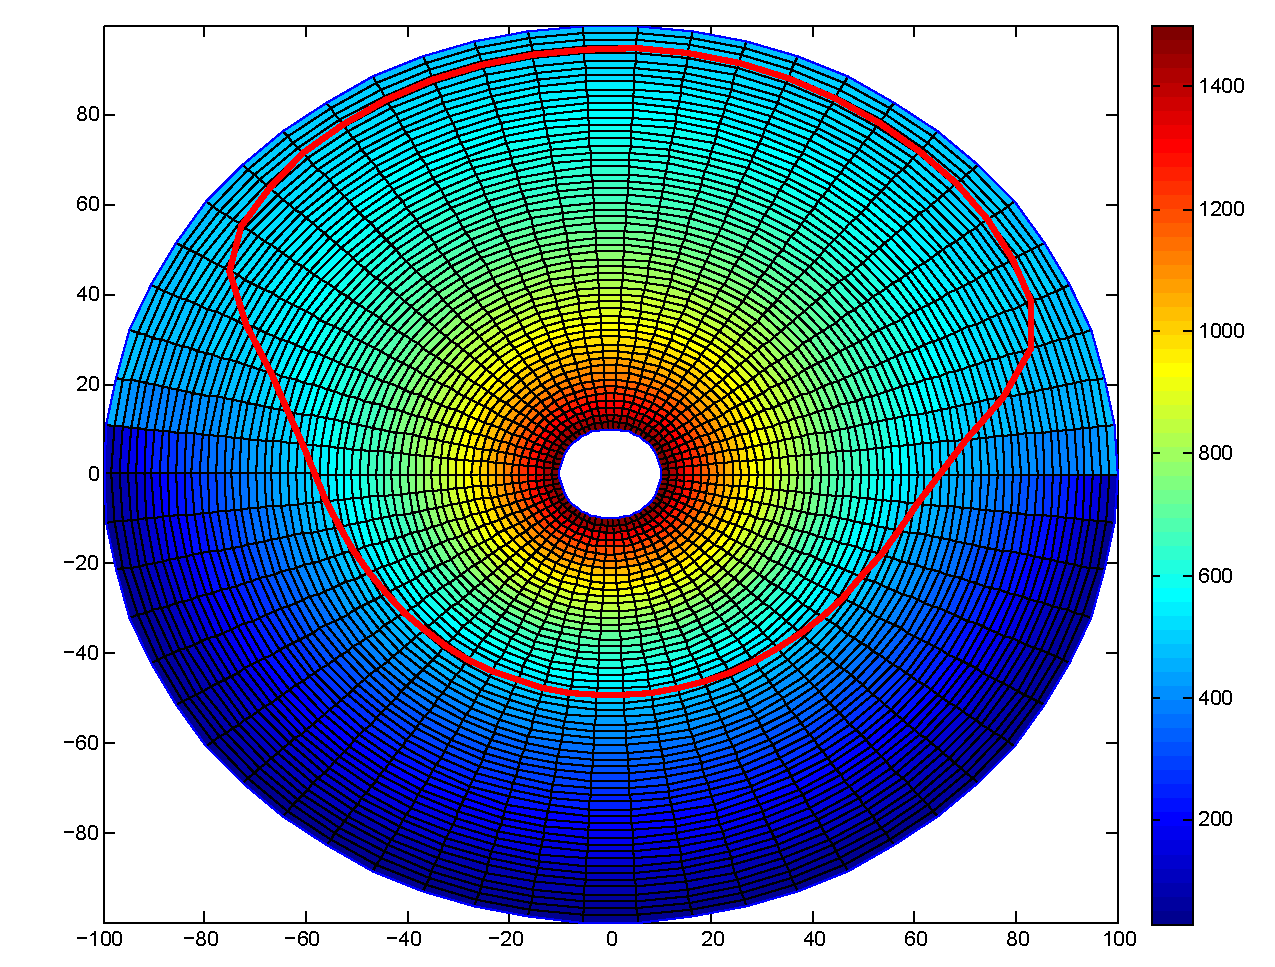
\includegraphics[width=0.75\textwidth]{figures/friocalor-isoterma-mn19.pdf}
\end{figure}

Un caso más interesante es el de la figura \ref{exp1-hfc}, donde la temperatura no es igual en todos los ángulos medidos. En el gráfico del horno se puede ver cómo la parte superior está más caliente que la inferior, y cómo la isoterma se va adaptando, moviendose entre casillas de colores muy similares, en la escala de la derecha podemos ver que el color por donde pasa la isoterma está muy cerca del color de la temperatura correspondiente a $500$.

~

\clearpage
\subsection{Análisis de performance}
\subsubsection{Medición de ciclos de procesador}

Para realizar las mediciones y comparaciones, en vez de medir los tiempos de inicio y final, utilizamos un método sugerido por Intel [Intel-1]\footnote{El paper sugiere más técnicas además de las que utilizamos nosotros para mejorar el monitoreo de performance: Correr el programa en un módulo de kernel sin desalojo y medir cuánto overhead tiene la llamada a rdtsc. Eso es útil cuando se desea una granularidad extrema de menos de 1000 cicos de procesador, nosotros no necesitamos tanta granularidad}, contando los ciclos de procesador utilizando la instrucción de procesador \textbf{RDTSC}. Tuvimos en cuenta las siguientes cosas:

\begin{itemize}
    \item Todas las mediciones fueron realizadas 10 veces, y luego se promediaron los valores
    \item Se corrieron los experimentos en un sistema multicore
    \item En vez de realizar una llamada a función, utilizamos una macro que usa inline-assembly para diminuir el overhead de realizar la medición en sí.
    \item Creamos una barrera de ejecución con la instrucción lfence para evitar que el procesador ejecutara instrucciones fuera de orden (es decir, para evitar que el procesador ejecutara rdtsc antes de haber terminado de ejecutar el programa). 
\end{itemize}

Consideramos que todos esos detalles nos brindan el nivel de precisión necesario para las mediciones del problema. 

En un sistema multiproceso como Linux es posible que no todos los ciclos de procesador sean destinados a nuestro proceso, tratamos de mitigar eso realizando los experimentos varias veces y luego promediando los ciclos insumidos, también ayuda el hecho de ejecutar el programa en un sistema multicore.

Decidimos utilizar una macro inline assembly y rdtsc ya que hay un overhead significante en llamar a funciones, y obtener el tiempo. Es posible que al obtener el tiempo actual se realize una \textbf{syscall} y esto desaloje nuestro proceso\footnote{A menos que el kernel implemente vDSO para la función de obtener el tiempo.}. Es cierto que para instancias grandes del problema, una diferencia de medio segundo es casi despreciable, pero consideramos que realizar las mediciones de esta forma disminuyen el error sin mucho esfuerzo.

Finalmente, la forma en la que utilizamos todo esto es: El programa cuenta los ciclos de reloj antes y despues de resolver el sistema (llamando a la macro que se puede encontrar en el archivo \textbf{tiempo.h}), los ciclos insumidos es el valor absoluto de la diferencia entre ciclos iniciales y finales. \footnote{notar que dado que usamos precisión de 64 bits, sólo es posible que haya overflow si la computadora estuvo prendida por más de 500 años}. 

\subsubsection{Benchmarks}


Realizamos una serie de pruebas para analizar la performance de la resolución del sistema. Hicimos las pruebas en las tres instancias descriptas previamente. Realizamos los tests variando la cantidad de puntos de discretizaci\'on que utilizamos, variando el $n$ (cantidad de \'angulos o sensores), el $m$ (cantidad de radios) y $n$ y $m$ al mismo tiempo. Medimos los resultados contando los ciclos de procesador insumidos. Por cada test corrimos $10$ repeticiones del mismo y luego promediamos los resultados, a modo de amortizar los ciclos de más por ser desalojados del scheduler. 

~

Esperamos que cada uno de los distintos escenarios insuman cantidades muy cercanas de ciclos en su resolución, ya que los valores de los datos deber\'ian ser irrelevantes para el tiempo de procesamiento. Adem\'as, el tiempo de procesamiento deber\'ia seguir un comportamiento cúbico en función de la entrada, ya que es esa es la complejidad del algoritmo utilizando eliminaci\'on Gausseana.

\begin{SCfigure}[1][ht!]
\sidecaptionvpos{figure}{t}
  \caption{ Se pueden observar los resultados de las primeras tres pruebas. Variamos $n$ (cantidad de angulos o sensores) en los tres escenarios que presentamos anteriormente utilizando eliminación Gausseana para resolverlos. Como se puede visualizar, el insumo de ciclos es cúbico en función de la cantidad de ángulos y la resolución de los tres escenarios insumió una cantidad muy cercana de ciclos, que es lo que estabamos esperando. \newline \newline}
  \includegraphics[width=0.6\textwidth]{../src/experimentacion/PDFs/sensores.pdf}
\end{SCfigure}

\begin{SCfigure}[1][ht!]
\sidecaptionvpos{figure}{t}
  \caption{ Al igual que la figura anterior, se puede observar exactamente el mismo comportamiento cuando solamente variamos $m$: un insumo de ciclos cúbico e insumos cercanos para los tres escenarios. \newline \newline \newline \newline \newline \newline \newline \newline}
  \includegraphics[width=0.6\textwidth]{../src/experimentacion/PDFs/radios.pdf}
\end{SCfigure}

\begin{SCfigure}[1][ht!]
\sidecaptionvpos{figure}{t}
  \caption{ Esta figura, si bien sigue la misma tendencia que las anteriores, es un poco distinta. Debido a la variación de ambos parametros la curva es mucho más cócava que en las experimentaciones anteriores. Sin embargo, los tres escenarios siguen insumiendo una cantidad similar de ciclos en cada instancia, que es lo que esperabamos ver.\newline \newline \newline \newline}
  \includegraphics[width=0.6\textwidth]{../src/experimentacion/PDFs/ambos.pdf}
\end{SCfigure}

\newpage
\subsection{Factorización LU vs Eliminación Gaussiana}

En esta sección compararemos la performance de los dos métodos de resolución utilizados. Dado que LU factoriza una sola vez la matriz, resolver el mismo sistema cambiando solo las mediciones implica un menor costo que resolver todo el sistema nuevamente (cosa que sucede con el método de eliminación Gaussiana). Basándonos en este razonamiento, esperamos conseguir una mejora de performance por parte del método LU cuando hay que resolver varias instancias del mismo sistema.


Proponemos dos experimentos, el primero consiste calcular la isoterma para muchas instancias del mismo horno, pero variando la temperatura de los sensores, simulando un efecto de 'paso del tiempo', en donde las paredes externas del horno comienzan a calentarse desde un estado inicial con temperatura $0$. La evolución del estado del horno se puede apreciar en la figura \ref{exp2-hornos}. En la figura \ref{compbench-glu} mostramos la comparativa de ciclos insumidos por LU y Gauss, confirmando que conviene realizar LU cuando queremos analizar más de una instancia. Sin embargo, la cantidad de ciclos insumidos para la primer iteración es similar: el método LU debe factorizar la matriz y eso lleva casi lo mismo que el método de eliminiación gaussiana. 


El segundo experimento trata de mostrar cómo varían la performance en función del tamaño del sistema y de las iteraciones. Simulamos varios sistemas como el anterior (un horno calentándose), pero en cada sistema aumentamos la cantidad de radios de la discretización y la cantidad de instancias. Con esto esperamos poder mostrar que luego de resolver la primer instancia, el proceso de resolución de las instancias siguientes es mucho más rápido con LU que con Gauss. Esto se puede ver en la figura \ref{compbench-extra}.

~

\begin{figure}[!htb]
    \caption{Evolución del horno en función del tiempo. Se ve cómo la isoterma de $500$ grados se acerca hacia el borde del horno, hasta que lo supera.}
    \label{exp2-hornos}
\centering
\minipage{0.5\textwidth}

  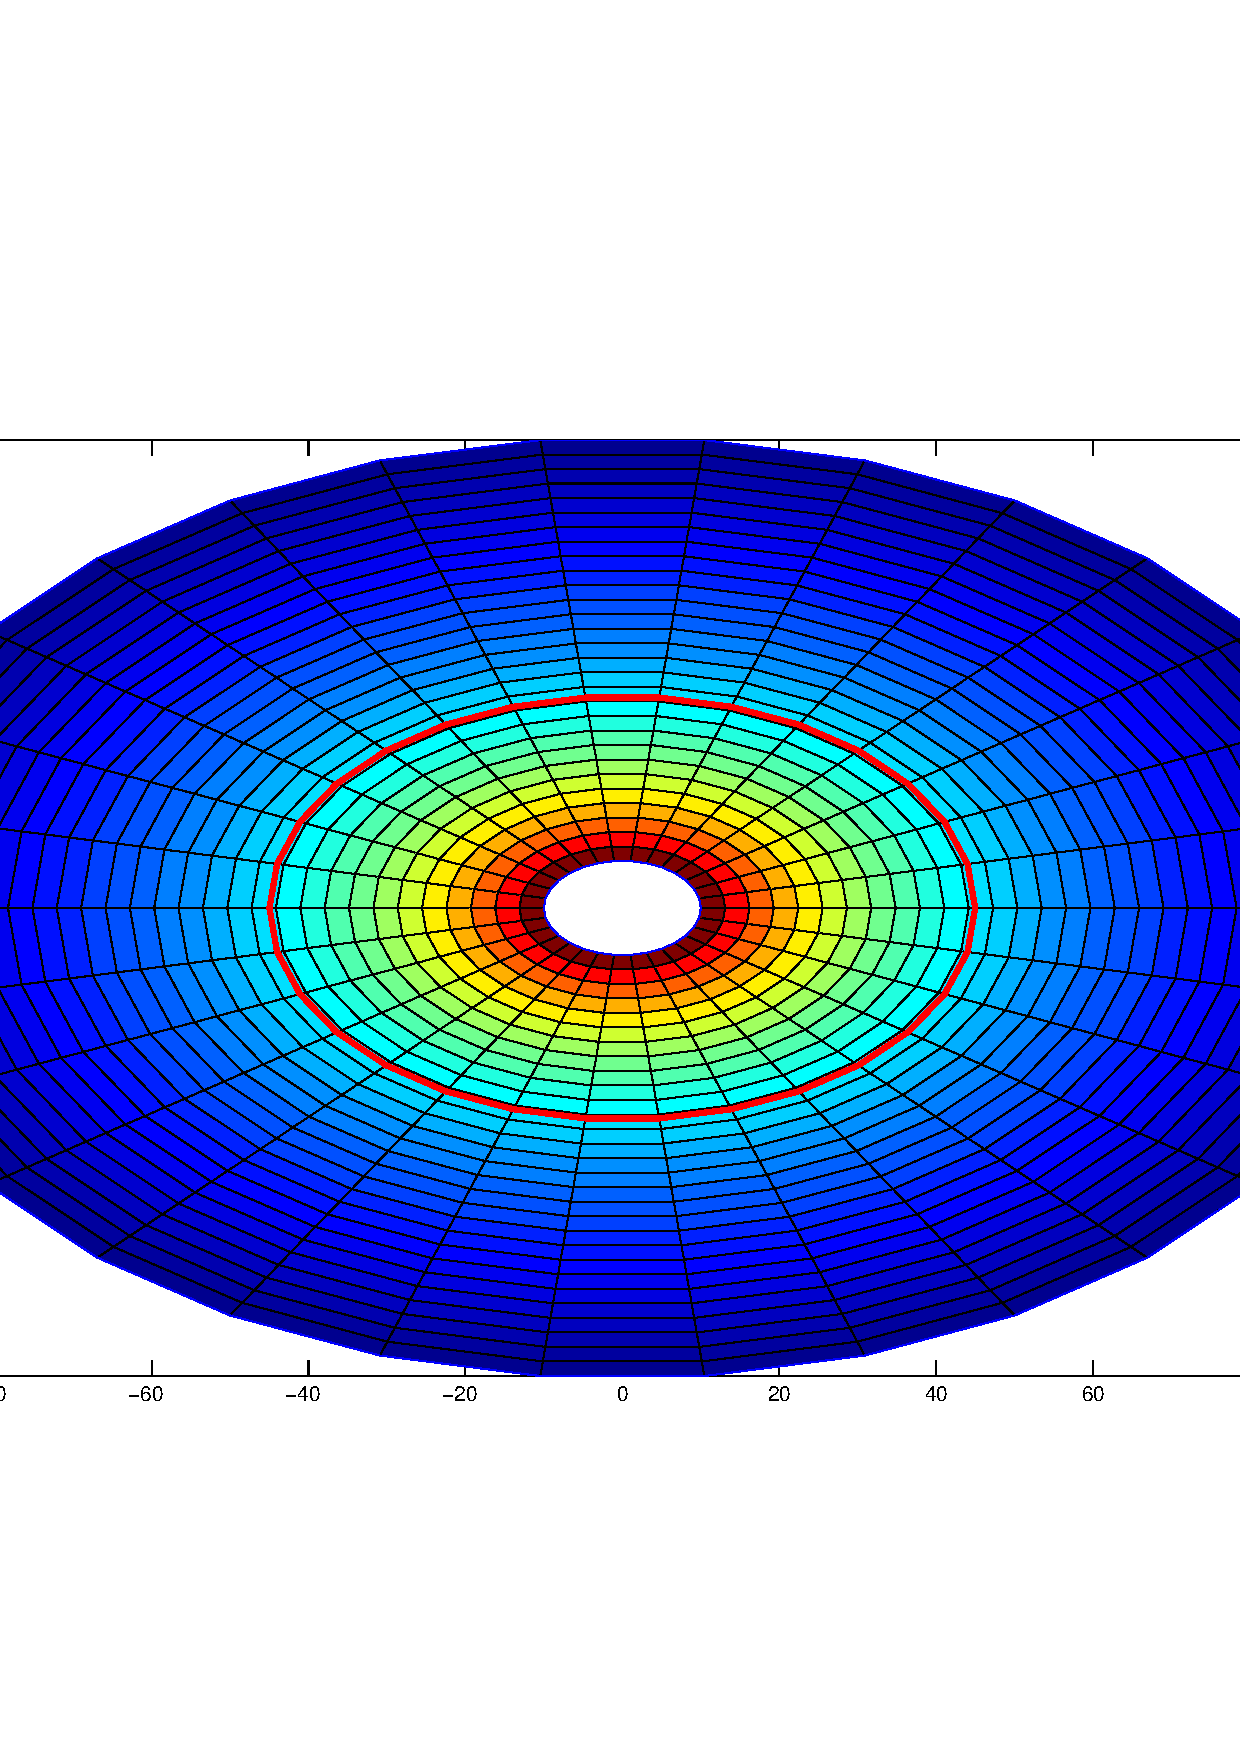
\includegraphics[width=1\textwidth]{figures/exp2-1.pdf}

\endminipage\hfill
\minipage{0.5\textwidth}

  \includegraphics[width=1\textwidth]{figures/exp2-2.pdf}

\endminipage\hfill
\minipage{0.5\textwidth}

  \includegraphics[width=1\textwidth]{figures/exp2-3.pdf}

\endminipage\hfill
\minipage{0.5\textwidth}

  \includegraphics[width=1\textwidth]{figures/exp2-4.pdf}

\endminipage\hfill
\end{figure}

\clearpage

\begin{SCfigure}[1][ht!]
\sidecaptionvpos{figure}{t}
  \caption{ Se puede observar la comparaci\'on de performance entre eliminaci\'on Gausseana (GE) y factorizaci\'on LU con 20 instancias seguidas del mismo sistema. Como se visualiza, en la primera resoluci\'on del sistema el insumo de ciclos es casi el mismo, mientras que en las consecuentes la factorizaci\'on LU toma mucha ventaja con respecto a la eliminaci\'on Gausseana. Los resultados muestran un crecimiento lineal en funci\'on de la cantidad de instancias, ya que al haber fijado  el $n$ y el $m$ el insumo de ciclos en la resoluci\'on de una instancia es constante.\newline}
  \includegraphics[width=0.6\textwidth]{../src/experimentacion/PDFs/compbench.pdf}
  \label{compbench-glu}
\end{SCfigure}

\begin{SCfigure}[1][ht!]
\sidecaptionvpos{figure}{t}
\caption{ En esta última experimentaci\'on intentamos realizar una comparativa que muestre mas claramente la diferencia de complejidad entre eliminaci\'on Gausseana y factorizaci\'on LU. Para ello realizamos $20$ iteraciones en las cuales $n=10$ para todas y $m$ era incrementado de a dos unidades en cada iteraci\'on (con un valor inicial de $10$). A la par de los incrementos de $m$ era incrementado $ninst$ de forma tal de que en las primeras iteraciones se pudiese observar con el algoritmo de LU un comportamiento mas cercano a una complejidad de $\mathcal{O}(n^3)$, mientras que en las ultimas iteraciones donde $ninst > 100$ el factor $n^2$ tomar\'ia mas importancia que la primera pero \'unica resoluci\'on con complejidad $n^3$.}
    \label{compbench-extra}
  \includegraphics[width=0.6\textwidth]{../src/experimentacion/PDFs/compbench-extra.pdf}
\end{SCfigure}



\clearpage
\section{Demostración}
  \textbf{Proposición: } Sea $A \in \mathbb{R}^{nxn}$ la matriz obtenida para el sistema definido por $(6) - (9)$. Es posible aplicar eliminación Gaussiana sin pivoteo.

\subsection{Aclaraciones}

En las siguientes demostraciones, se usará la notación $A^{(k)}$ para referirse a la matriz resultante de aplicar k pasos de eliminación gaussiana en A, para algún $k \in \mathbb{N}$

\subsection{Demostración de la propiedad}
\textbf{Lema 0:} Sea $A \in \mathbb{R}^{nxn}$ una matriz cuyas filas son \textit{linealmente independientes} (LI), no existe una columna de A con elementos todos nulos.

\textbf{Lema 1:} Sea $A \in \mathbb{R}^{nxn}$ una matriz cuyas filas son LI, vale que  $\forall i, j \in [1, n], i \neq j$ la matriz resultante de restar un múltiplo cualquiera de la fila i a la fila j tambien es LI.



\textbf{Lema 2:} Sea $A \in \mathbb{R}^{nxn}$ una matriz DDNE cuyas filas son LI, se puede hacer un paso de eliminación Gaussiana sin pivote.



\textbf{Lema 3:} Sea $A \in \mathbb{R}^{nxn}$ una matriz DDNE cuyas filas son LI, la submatriz resultante de aplicar un paso de la eliminación Gaussiana es DDNE.
\\

\textbf{Demostración:} Sea $A$ una matriz definida por $(6) - (9)$. Vale que $A$ es una matriz cuadrada que es \textit{diagonal dominante no estricta} (DDNE) cuyas filas son LI. 

Luego, por el \textbf{Lema 0}, \textbf{Lema 1} y el \textbf{Lema 2} puedo aplicar un paso de la eliminación gaussiana conservando la independencia lineal. 
Por el \textbf{Lema 3} vale que la matriz resultante sigue siendo DDNE y LI, cumpliendo de nuevo las hipótesis originales. Aplicando este paso $n$ veces, se obtiene la matriz $A^{(n)}$ sin pivotear. $\blacksquare$


\subsubsection{Demostración del Lema 0}
Sea $A \in  \mathbb{R}^nxn$ una matriz cuyas filas son linealmente independientes.

Asumamos que A tiene una columna de elementos todos nulos. Entonces, $A^{t}$ tiene una fila de elementos todos nulos.

Por lo tanto $det( A^{t}) = 0$ [Hefferon-1]$\Rightarrow det(A) = 0$ [Jeronimo-1]$\Rightarrow$ Las filas de A son linealmente dependientes[Jeronimo-2]. 

El absurdo provino de suponer que la matriz A, teniendo filas linealmente independientes, puede tener una columna de elementos todos nulos.
\subsubsection{Demostración del Lema 1}
Sea $A \in \mathbb{R}^{nxn}$. Que sus filas sean LI implica que:
\begin{equation} 
\lambda_{1} f_{1} + ... + \lambda_{n}f_{n}  = 0 \Leftrightarrow \lambda_{p} = 0,  \forall p \in [1..n]
\end{equation} 
\\
Supongamos ahora que realizo la operación de restarle a la fila j-ésima de A, un m\'ultiplo de la fila i-ésima de A. Una combinación lineal de las filas de la matriz resultante, llam\'emosla A', podr\'ia escribirse en función de las filas originales como:
\\
\begin{equation} 
\lambda_{1} f_{1} + ... + \lambda_{i} f_{i} + ... + \lambda_{j} f_{j} - k  \lambda_{i} f_{i} + ... + \lambda_{n}f_{n}  =
\end{equation} 
\\
\begin{equation} 
\lambda_{1} f_{1} + ... + ( \lambda_{i} - k) f_{i} + ... + \lambda_{j} f_{j} + ... + \lambda_{n}f_{n}  =
\end{equation} 
\\
Si ahora tomamos $ \lambda'_{i} = \lambda_{i} - k $ como coeficiente, podemos obtener la siguiente expresi\'on, que es equivalente a la que obtuvimos originalmente de los vectores de A. 

\begin{equation} 
\lambda_{1} f_{1} + ... +  \lambda_{i}' f_{i} + ... + \lambda_{n}f_{n} =  \Leftrightarrow \lambda' = 0 \wedge  \lambda_{i} = 0 \forall \lambda \in [1 .. n]
\end{equation} 

Con lo cual si las filas de A son linealmente independientes,  las de A' tambi\'en lo son.
\subsubsection{Demostración del Lema 2}
Si $A$ es DDNE, entonces $\forall i, j \in [1, n], |a_{jj}| \geq|a_{ij}|$.

Como la matriz tiene filas LI y es cuadrada, por \textbf{Lema 0}, no existe una columna de elementos todos nulos. 

Luego, $\forall j \in [1, n] \exists i_0 \in [1, n] / |a_{i_0 j}| > 0$, finalmente, como es DDNE $\forall i \in [1, n], |a_{ii}| \geq |a_{i_0 j}| > 0$. 

Esto significa que los elementos de la diagonal son no nulos, y, por lo tanto, se puede realizar un paso de la eliminación Gaussiana sin necesidad de pivotear.

\subsubsection{Demostración del Lema 3}
Quiero ver que al hacer eliminación Gaussiana, la submatriz resultante no pierde su propiedad de DDNE. Dada una matriz  $A^{(0)} \in \mathbb{R}^{nxn}$ y que se realizó un paso de la factorización de Gauss, siendo la matriz resultante nombrada $A^{(1)}$. En tal caso, un elemento de $A^{1}$ se escribe:
\\
\begin{equation*}
\centerline{$|a^{(1)}_{ij}| = |a^{(0)}_{ij} - \frac{a^{(0)}_{i1}}{a^{(0)}_{11}}  a^{(0)}_{1j}|$}
\end{equation*}
Y la propiedad que queremos probar se escribe:
\\
\begin{equation*} 
\sum_{i=2, i \neq j}^{n}  |a^{(1)}_{ij}| \leq |a^{(1)}_{jj}| 
\end{equation*}
De ahora en mas se evitara usar los supraindices por cuestiones de simplicidad. Reemplazando (10) en (11) vale que
\begin{equation*} 
\sum_{i=2, i \neq j}^{n}  |a_{ij} - \frac{a_{i1}}{a_{11}}  a_{1j}|  \leq
\end{equation*}
\begin{equation*} 
\sum_{i=2, i \neq j}^{n}  |a_{ij}| + \sum_{i=2, i \neq j}^{n}  |\frac{a_{i1}}{a_{11}}  a_{1j}|  =
\end{equation*}
\begin{equation*} 
-|a_{1j}| + \sum_{i=1, i \neq j}^{n}  |a_{ij}| + \sum_{i=2, i \neq j}^{n}  |\frac{a_{i1}}{a_{11}}  a_{1j}|
\end{equation*}
Pero como $A^{(0)}$ es DDNE
\begin{equation*} 
\sum_{i=1, i \neq j}^{n}  |a_{ij}|  \leq |a_{jj}| \Rightarrow (18) \leq  -|a_{1j}| + |a_{jj}| + \sum_{i=2, i \neq j}^{n} | \frac{a_{i1}}{a_{11}} a_{1j}| = 
\end{equation*}
\begin{equation*} 
|-a_{1j}| + |a_{jj}| + | \frac{a_{1i}}{a_{11}}| \sum_{i=2, i \neq j}^{n}  |a_{i1}|
\end{equation*} 

\newpage

Otra vez, usando que $A^{(0)}$ es DDNE
\begin{equation*} 
\sum_{i=2}^{n}  |a_{i1}|  \leq |a_{11}| \Rightarrow
\end{equation*}
\begin{equation*} 
\sum_{i=2, i \neq j}^{n}  |a_{i1}| +|a_{j1}| \leq |a_{11}|
\end{equation*}
\begin{equation*} 
\sum_{i=2, i \neq j}^{n}  |a_{i1}|  \leq |a_{11}| - |a_{j1}|
\end{equation*}

Esto implica que
\begin{equation*} 
(20) \leq - |a_{ij}| + |a_{jj}|  + |\frac{a_{1j}}{a_{11}}|(|a_{11}| - |a_{j1}|)
\end{equation*}
\begin{equation*} 
= |a_{jj}| - | \frac{a_{1j}}{a_{11}}| |a_{j1}| \leq |a_{jj} - \frac{a_{1j}}{a{11}} a_{j1}| = |a_{jj}^{(1)}|
\end{equation*}


\section{Conclusiones}
  Mediante los resultados obtenidos por la experimentaci\'on, pudimos concluir que la factorizaci\'on LU es igual (para los casos de una instancia) o m\'as performante (para los casos de mas de una instancia) que la eliminaci\'on Gausseana. 

~

El an\'alisis de performance deja en evidencia que efectivamente la eliminaci\'on Gausseana tiene una complejidad de $\mathcal{O}((nm)^3)$ para toda iteraci\'on mientras que la factorizaci\'on LU tiene una complejidad de $\mathcal{O}((nm)^3)$ para la primera resoluci\'on mientras que para sucesivas resoluciones tiene una complejidad de $\mathcal{O}((nm)^2)$.

~

En un sistema de control de temperaturas real, en donde tendr\'iamos que dar una estimaci\'on a cada instante de la temperatura del horno y del calculo de la isoterma para poder prevenir accidentes, la factorizaci\'on LU supone una mejor manera de hacerlo. ya que como el sistema no cambiara la cantidad de sensores (ya que son piezas de hardware y demandar\'ia una reinstalaci\'on de los mismos) tampoco lo har\'a la matriz asociada al sistema. Es por ello que hasta podr\'iamos hacer el calculo de la matriz de antemano, de alguna forma hardcodearlo para que todo funcione aun mas r\'apido y luego resolver el sistema y dar las estimaciones cuando los datos de los sensores lleguen.
 

\clearpage
\section{Apéndice A: Implementación}
    \subsection{Implementación en C++}

Proveemos un programa de computadora para resolver instancias de este problema, mediante distintos métodos, a saber, Eliminación gaussiana y Factorización LU. El código fuente del programa se encuentra adjunto a este documento.

El código está en lenguaje C++11 con una extensión en Assembler de la arquitectura Intel x86-64 para contar los ciclos de procesador insumidos, esto fue utilizado en la sección Experimentación y allí se encuentra una explicación.

Para generar el binario se necesita:

\begin{itemize}
    \item GNU Make para compilar y generar el binario
    \item El compilador g++ de GNU, versión 4.6.3 (Se puede utilizar otro compilador, pero este debe soportar el estándar de C++11 y soporte inline-assembly con sintaxis Intel.
\end{itemize}

Utilizando GNU Make se puede generar un binario compatible con arquitecturas Intel x86-64. Para ello, hay que ejecutar:

\begin{verbatim}
    make main
\end{verbatim}

Esto generará un archivo ejecutable llamado \textbf{tp}, para ejecutarlo, se deben brindar los siguientes parámetros:

\begin{itemize}
    \item \textbf{archivo\_in} el nombre de un archivo que describa un sistema con un formato parseable, el mismo será descripto más adelante (formato entrada).
    \item \textbf{archivo\_out} nombre del archivo donde se desee guardar el sistema resuelto, con un formato que también será descripto más adelante (formato salida)
    \item \textbf{modo} Modo de resolución 0 para Gauss, 1 para LU
    \item \textbf{archivo\_iso} (opcional) nombre del archivo en donde se desee guardar la información de la isoterma, con un formato que será descripto más adelante (formato isoterma)
\end{itemize}

Por ejemplo, se puede ejecutar el binario como:

\begin{verbatim}
    ./tp archivo.in archivo.out 1 archivo.isoterma
\end{verbatim}

Donde archivo.in es un archivo existente y archivo.out y archivo.isoterma pueden no existir y serán sobreescritos.

\subsubsection{Formatos de Archivos}

La especificación del formato de entrada y formato salida se encuentra en el Apéndice B - Enunciado.
La especificación del formato de la isoterma es: para un horno de n sensores y k instancias, un archivo con $k * n$ líneas, con un número real en cada línea, donde las línea $i$ contiene el radio de la isoterma para la instancia $[\frac{i}{n}]$ del sensor $i \% n$ (que representa 'el resto de dividir a $i$ por $n$).

\subsubsection{Scripts para MATLAB y Python}

También proveemos scripts para resolver el sistema en MATLAB y Python. Estos scripts fueron utilizados para prototipar el programa en C++ y encotrar errores en las operaciones. Los mismos se encuentran dentro de la carpeta 'exp' del directorio de archivos provisto. Para ejecutar estos archivos es necesario poseer los programas MATLAB y Python 2.7 (también la librería scipy). 

\subsubsection{Generación de Experimentos}

Proveemos también los scripts utilizados para generar  y correr los experimentos. Estos se encuentran dentro de la carpeta 'experimentacion'. Se necesita poseer bash alguna shell compatible y el programa Go, compilador oficial del lenguaje de programación Go (algunos de los programas fueron hechos en este lenguaje). Es necesario compilar el tp y los programas y ponerlos en las carpetas donde están los scripts.

\clearpage
\section{Bibliografía}
    \begin{verbatim}
    [Intel-1]:
        titulo: How to Benchmark Code Execution Times 
                on Intel IA-32 and IA-64 Instruction Set Architectures
        url: 
        http://www.intel.com/content/dam/www/public/
        us/en/documents/white-papers/ia-32-ia-64-benchmark-code-execution-paper.pdf

    [Jeronimo-1]:
        titulo: Algebra Lineal
        autores:Gabriela Jeronimo, Juan Sabia y Susana Tesauri
        ISSN: 1851-1317
        Capítulo 5, pág 115.

    [Jeronimo-2]:
        titulo: Algebra Lineal
        autores:Gabriela Jeronimo, Juan Sabia y Susana Tesauri
        ISSN: 1851-1317
        Capítulo 5, pág 119.

   [Hefferon-1]:
        titulo: Linear Algebra
        autor: James Hefferon
        url: http://joshua.smcvt.edu/linearalgebra
        Capítulo 4, pág 322.
\end{verbatim}
\end{document}
